


\section{Referent implementation}
\label{sec:implementation}

We implement the \acro{TSMS} and \acro{MTSMS} models with Python
\cite{python:doc2} programming language. It is a referent
implementation in order to show how a system can be developed from the
models, therefore it has fidelity to the algebraic model defined in
Section~\ref{sec:model:TSMS} and \ref{sec:MTSMS} but has not extended
\acro{DBMS} components, as would be query optimisation or
transaction management.

The two models of \acro{TSMS} and \acro{MTSMS} are implemented
respectively as two separated Python libraries: Pytsms and
RoundRobinson.  RoundRobinson has a strong dependency on Pytsms
following the \acro{MTSMS} being defined based on \acro{TSMS}.  The
code of this implementation can be found at
\cite{llusa:roundrobinson}.

We design the implementation concepts with object orientation, being a
clear mapping between model and implemented objects. Unified Modeling
Language (\acro{UML}) diagrams are used for defining the classes
structure, mainly to show the relationships among objects.  Operations
are implemented as object methods, which are not show in \acro{UML}
diagrams for space reasons.


% The development of this implementation is free software and can be found at our version control system
% \url{http://escriny.epsem.upc.edu/svn/rrb//src/roundrobinson/tags/0.3/}.


\subsection{Pytsms}

Pytsms is the referent implementation for the model concepts of
measure, time series and temporal representation function.  Figure
\ref{fig:implementacio:pytsms-uml} shows the relationships among these
objects in a \acro{UML} diagram. A \emph{TimeSeries} object is an
aggregation of \emph{Measure} objects. \emph{TimeSeries} and
\emph{Representation} objects have a relation of association, that is
each \emph{TimeSeries} has a default representation and a
\emph{Representation} operates over a \emph{TimeSeries}.

%\tikzsetnextfilename{fig_pytsms_uml}
\begin{figure}[tp]
  \centering
  %  \begin{tikzpicture}

  %Timeseries
  \umlsimpleclass[x=0,y=0] {TimeSeries}{}{}

  % Measure
  \umlclass[x=-1.5,y=-2] {Measure}{}{}
  \umluniaggreg[mult=0..*]  {TimeSeries}{Measure}
  %\umlclass[x=-5.2,y=-2] {MFloat}{}{}
  %\umlclass[x=-2.8,y=-2] {MChar}{}{}
  %\umlinherit {MFloat}{Measure}
  %\umlinherit {MChar}{Measure}

  %Repr
  \umlclass[x=3.5] {Representation}{}{} %,type=abstract
  \umlassoc[mult1=1,mult2=1]  {TimeSeries}{Representation}
  \umlclass[x=2.5,y=-2] {Zohe}{}{}
  \umlclass[x=4.5,y=-2] {Dd}{}{}
  \umlinherit {Zohe}{Representation}
  \umlinherit {Dd}{Representation}

  %Associacions
  \umlclass[x=-1.25,y=-4] {RegularProp}{}{}
  \umluniassoc  {TimeSeries}{RegularProp}
  \umlclass[x=1.25,y=-4] {Storage}{}{}
  \umluniassoc {TimeSeries}{Storage}

  %Dependencies
  \umlemptypackage[x=4,y=-5]{Matplotlib}
  \umldep{Zohe}{Matplotlib}
  \umldep{Dd}{Matplotlib}


  \end{tikzpicture}

  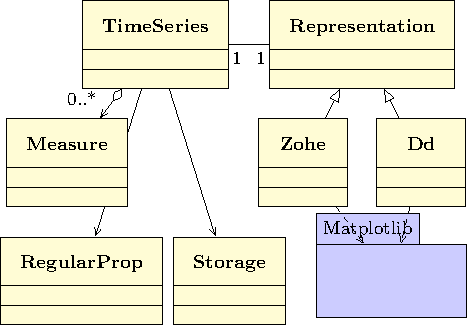
\includegraphics{fig_pytsms_uml.pdf}
  \caption{Pytsms \acro{UML} class diagram}
  \label{fig:implementacio:pytsms-uml}
\end{figure}




A \emph{TimeSeries} object has a huge amount of methods, we classify
them based on their functionality. Firstly, a \emph{TimeSeries}
includes methods for manipulating the structural model, we implement
\emph{TimeSeries} as a subclass of the predefined \emph{Set} Python
type. Secondly, there are methods for set, sequence and temporal
function operators as described in Section~\ref{sec:model:operations}.
Thirdly, complementary operations for \emph{TimeSeries} are grouped
into two visitor objects: \emph{RegularProp} groups the regularity
operation definitions and \emph{Storage} has methods for storing and
retrieving time series from file system. Visitor is a pattern design
that allows new functionality to be added to objects without modifying
the objects
\cite{ziade08:expert_python_programming:visitor,martin02:visitor}.


Figure \ref{fig:implementacio:pytsms-uml} shows two specialisations
for \emph{Representation}. We show the two representations \emph{Zohe}
and \emph{Dd} in Section~\ref{sec:model:tfunc}. Basically, each
particular \emph{Representation} has the graph and the temporal
interval operation definition. Furthermore, there is also a method for
plotting coherently the time series to its representation; for which
we use the Python \emph{Matplotlib} library.



\begin{example}
  \label{ex:pytsms:example}
  We define in Pytsms the two time series $S1$ and $S2$ from
  Example~\ref{ex:model:s1s2} and we apply different operations:
  union, temporal union, concatenation, closed interval, \zohe{}
  temporal interval, \zohe{} temporal selection, and the test of
  regular property. Note that \emph{Measure} is abbreviated to
  \emph{m}.
{\small
\begin{verbatim}
# Import the required objects
>>> from pytsms import TimeSeries, Measure as m
>>> from pytsms.representation import Zohe
>>> from pytsms.properties import isRegular

# Define the two time series
>>> s1 = TimeSeries([m(1,1),m(3,1),m(4,0),m(5,1)])
>>> s2 = TimeSeries([m(2,2),m(3,2),m(4,0),m(6,2)])

# Manipulate the two time series
>>> s1.union(s2)
TimeSeries([m(1,1), m(2,2), m(3,1), 
            m(4,0), m(5,1), m(6,2)])
>>> s1.union_temporal(s2)
TimeSeries([m(1,1), m(2,2), m(4,0), m(5,1), m(6,2)])
>>> s1.concatenate(s2) 
TimeSeries([m(1,1), m(3,1), m(4,0), m(5,1), m(6,2)])
>>> s2.interval_closed(2,5)
TimeSeries([m(2,2), m(3,2), m(4,0)])
>>> s2.interval_temporal(2,5,Zohe)
TimeSeries([m(3,2), m(4,0), m(5,2)])

# Check for regularity
>>> s2.accept(isRegular())
False
# regularise to {0,2,4} by Zohe method
>>> r2 = s2.selection_temporal(range(0,6,2),Zohe)
>>> r2
TimeSeries([m(0,2), m(2,2), m(4,0)])
>>> r2.accept(isRegular())
True
\end{verbatim}
}
\end{example}





\subsection{RoundRobinson}


RoundRobinson is the referent implementation for the model concepts of
multiresolution time series, resolution subseries, buffers, discs, and
attribute aggregate functions. Figure
\ref{fig:implementacio:roundrobinson-uml} shows the relationships
among these objects in a \acro{UML} diagram. A
\emph{MultiresolutionSeries} object is an aggregation of
\emph{Resolution} objects. A \emph{Resolution} is composed of one
\emph{Buffer} and one \emph{Disc}. Each \emph{Buffer} is associated to
one \emph{TimeSeries}, from the Pytsms library, and each \emph{Disc}
is associated to another \emph{TimeSeries}, which respectively are
$S_B$ and $S_D$ of the \acro{MTSMS} model. Furthermore, each
\emph{Buffer} is associated to one attribute aggregate function which
is realised by defining a Python \emph{Function} with two parameters:
a \emph{TimeSeries} (\emph{s}) and a consolidation time interval
(\emph{i}).



%\tikzsetnextfilename{fig_roundrobinson_uml}
\begin{figure}[tp]
  \centering
  %\begin{tikzpicture}

  %MultiTimeseries
  \umlsimpleclass[x=0,y=0] {MultiresolutionSeries}{}{}  
  %\umlclass[x=-4,y=0] {Set}{}{}
  %\umlinherit{MultiresolutionSeries}{Set}
  %Components 
  \umlclass[x=0,y=-2] {Resolution}{}{}
  \umluniaggreg  {MultiresolutionSeries}{Resolution}
  %SubComponents 
  \umlclass[x=-1.2,y=-4] {Buffer}{}{}
  \umlclass[x=1.2,y=-4] {Disc}{}{}
  \begin{umlpackage}[x=-3,y=-6.6]{aggregators}
    \umlclass[template={s,i}] {Function}{}{}
  \end{umlpackage}
  \umlunicompo[mult=1]  {Resolution}{Buffer}
  \umlunicompo[mult=1]  {Resolution}{Disc}
  \umluniassoc[mult=1]  {Buffer}{Function}

  %TimeSeries
  \begin{umlpackage}[x=1,y=-6.5]{Pytsms}
    \umlclass{TimeSeries}{}{}  
  \end{umlpackage}
  \umluniassoc[mult=1]  {Buffer}{TimeSeries}
  \umluniassoc[mult=1]  {Disc}{TimeSeries}

  %Associacions
  \umlclass[x=-3.25,y=-2.7] {Storage}{}{}
  \umluniassoc {MultiresolutionSeries}{Storage}
  \umlclass[x=-3.5,y=-1] {Plot}{}{}
  \umluniassoc {MultiresolutionSeries}{Plot}

\end{tikzpicture}

  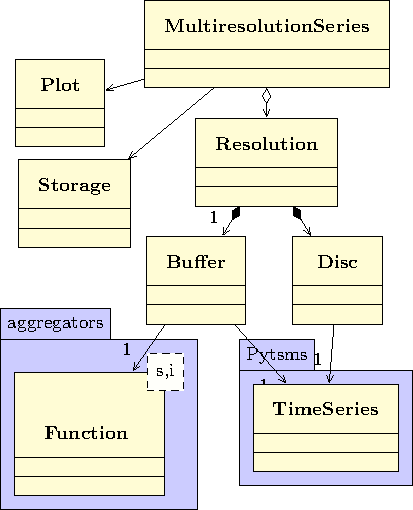
\includegraphics{fig_roundrobinson_uml.pdf}
  \caption{RoundRobinson \acro{UML} class diagram}
  \label{fig:implementacio:roundrobinson-uml}
\end{figure}



A \emph{MultiresolutionSeries} is a subclass of the predefined \emph{Set} Python
type. It has complementary operations that are grouped into two
objects: \emph{Storage} has methods for storing and retrieving
multiresolution time series from file system and \emph{Plot} has
methods for plotting the time subseries of the multiresolution schema.


A \emph{MultiresolutionSeries} has a method \emph{addResolution} for defining
the multiresolution schema structure by adding resolution
subseries. Every new resolution is configured by four parameters:
\emph{delta}, \emph{k}, \emph{f}, and \emph{tau} that create the
corresponding buffer and disc.  A \emph{MultiresolutionSeries} has methods
\emph{add}, \emph{consolidable}, and \emph{consolidate} that operate on
the corresponding methods of the contained resolution subseries.


A \emph{MultiresolutionSeries} can be queried by two methods:
\emph{seriedisc} and \emph{totalseries}. The \emph{seriedisc} returns
the \emph{TimeSeries} for the selected disc by parameters \emph{delta}
and \emph{f}. The \emph{totalseries} returns the \emph{TimeSeries}
that results from the concatenation of all \emph{seriedisc} ordered by
\emph{delta}.
% as there can not be repeated \emph{delta}, \emph{totalseries} has a
% parameter \emph{f} for selecting only \emph{discSeries} with a
% determined attribute aggregate function.

In a module \emph{aggregators} we have implemented some default
attribute aggregate functions, although users can define more as they
are Python \emph{Function} objects with parameters \emph{s} as a
\emph{TimeSeries} and \emph{i} as a pair of times like
\emph{[ti,tj]}. As instance we have defined the \zohe{} aggregate
functions from Section~\ref{sec:model:interpolador}, which basically
aggregate over the temporal interval
\verb|s.interval_temporal(ti,tj,Zohe)| shown in
Example~\ref{ex:pytsms:example}.


\begin{example}
  We define in Pytsms the time series $S$ and in RoundRobinson we
  define the multiresolution time series $M_\emptyset$ from
  Example~\ref{ex:model:smultiresolution}, we apply consolidation and
  we query the result.

{\small
\begin{verbatim}
#Importing the required objects
>>> from pytsms import TimeSeries, Measure as m
>>> from roundrobinson import MultiresolutionSeries
>>> from roundrobinson.aggregators import mean_zohe,maximum_zohe

#Defining the original time series
>>> s = TimeSeries([m(1,6),m(5,2),m(8,5),m(10,0),m(14,1),m(19,6),m(22,11),m(26,6),m(29,0)])

#Defining the multiresolution time series
>>> M = MultiresolutionSeries()
#Defining the multiresolution schema
>>> M.addResolution(delta=5,k=4,f=mean_zohe,tau=0)
>>> M.addResolution(delta=10,k=2,f=maximum_zohe,tau=0)

#Adding the measures
>>> for m in s: M.add(m)
#M is consolidable
>>> M.consolidable()
True
#Consolidating until no more consolidable
>>> while M.consolidable():
...    M.consolidate()

#Query the consolidated discs 
>>> M.seriedisc(5,mean_zohe)
TimeSeries([m(10,3), m(15,2), m(20,7), m(25,8)])
>>> M.seriedisc(10,maximum_zohe)
TimeSeries([m(10,6), m(20,11)])
#Query the total time series
>>> M.totalseries()
TimeSeries([m(10,3), m(15,2), m(20,7), m(25,8)])
\end{verbatim}
}
\end{example}





%%% Local Variables:
%%% TeX-master: "main"
%%% ispell-local-dictionary: "british"
%%% End:
